\levelstay{Driving} \label{sec:driving}

\leveldown{Capacitive driving}

We next consider driving signals applied to the circuit.
We attach a driving voltage source to our parallel LC through a capacitor $C_d$, as shown by the dotted elements in Fig.\,\ref{Fig:singleCircuit}.
The capacitor $C_d$ is required to prevent the driving circuit from completely ruining the coherence of the main circuit.
Without the capacitor, the loaded quality factor $Q_d$ of the main circuit due to the drive circuit would be \citeinternalref{loadedMode}
\begin{equation}
Q_d = R_d / Z_{LC} .
\end{equation}
With typical circuit impedances in the range 10's to 100's of Ohms, and RF source resistances of $50\,\Omega$\,\footnote{Commercial RF devices essentially \emph{all} use 50 \, $\Omega$ output impedance. This is simply due to the fact that a coaxial transmission line of reasonable size has near $50 \, \Omega$ impedance. The impedance depends logarithmically on geometric parameters and so cannot be significantly varied. 50$ \, \Omega$ has been chosen as a common standard.}, we have $Q_d \approx 1$ which is far too low to be useful in a quantum device.\footnote{The energy relaxation time of the circuit is $T_1 = Q_d / \omega$, so for a 1 GHz device $Q_l=1$ corresponds to $T_1=0.16 \, \text{ns}$.}

The coupling capacitor $C_d$ helps preserve the circuit coherence.
If $C_d$ is sufficiently small, its impedance $Z_{C_d} = 1/i\omega C_d$ is large and so the current flowing through $R_d$ is reduced.
Therefore, $C_d$ prevents the process by which energy from the oscillator gets into $R_d$ and is lost.
To be specific, in the limit $Z_{C_d} \gg R_d$ the loaded quality factor of the oscillator is \citeinternalref{loadedMode}
\begin{equation}
Q_l = \left( \frac{C}{C_d} \right)^2 \frac{Z_{LC}}{R_d} .
\end{equation}
Therefore, a small $C_d$ preserves the circuit's coherence.
However, decoupling the drive line from the driving voltage source with a small $C_d$ also limits the speed with which we can control the circuit, so a balance must be struck.
This issue is discussed in detail below.

We now turn back to formal analysis of the driven circuit.
Even before doing any formal analysis, we can make a qualitative prediction.
The main capacitor $C$ is shunted by the series combination of the coupling capacitor $C_d$, and the resistor $R_d$.
Because  $Z_{C_d} \gg R_d$ the impedance of the driving circuit is dominated by $C_d$ which simply adds in parallel with $C$.
Therefore, we expect the effective capacitance of the mode to be $C+C_d$.

Denoting the time dependent driving voltage by $V_d(t)$ and ignoring for now the resistance of the source, we work out Kirchhoff's equation of motion for the driven system, resulting in
\begin{equation}
\frac{1}{1+C/C_d} \dot{V}_d = \ddot{\Phi} + \frac{\omega_0^2}{1 + C_d/C} \Phi. \end{equation}
This is totally sensible: the drive strength increases as $C_d$ increases, and the resonance frequency of the LC mode has shifted due to the new capacitance.
This equation of motion is produced by the Lagrangian
\begin{equation}
\mathcal{L} = \frac{1}{2}C \dot{\Phi}^2 - \frac{1}{2L}\Phi^2 + \frac{1}{2} C_d \left( \dot{\Phi} - V_d \right)^2 \, .
\end{equation}
For the sake of identifying canonical coordinates we consider the case $V_d=0$, resulting in canonical variables
\begin{equation*}
  \Phi
  \qquad \textrm{and} \qquad
  p \equiv \frac{\partial \mathcal{L}}{\partial \dot{\Phi}} = \left( C + C_d \right) \dot{\Phi} \equiv Q
\end{equation*}
just as before, except that now the capacitance associated to the momentum $Q$ is $C+C_d$ instead of just $C$.
The Hamiltonian is
\begin{equation}
H = \frac{Q^2}{2 (C + C_d)} + \frac{\Phi^2}{2L} \, .
\end{equation}
Now we consider what happens when the drive turns on.
The term added to the Lagrangian by the drive is
\begin{equation}
  \mathcal{L}_d = \frac{1}{2}C_d V_d(t)^2 - C_d \dot{\Phi} V_d(t) \, .
\end{equation}
The first term is of no consequence as it does not involve the dynamical variables.
The second term couples the drive to the momentum $Q$, resulting in a Hamiltonian term
\begin{equation*}
H_d
  = C_d \dot{\Phi}V_d(t)
  = \frac{1}{1+C/C_d} Q V_d(t) \, . \label{eq:sec:driving:H_dVsCircuitParams}
\end{equation*}
Restricting to the lowest two levels, we can rewrite $H_d$ as
\begin{align}
H_d
&= \frac{V_d(t)}{1 + C/C_d} \left(
{\begin{array}{cc}\bbraket{0}{Q}{0} & \bbraket{0}{Q}{1} \\ \bbraket{1}{Q}{0} & \bbraket{1}{Q}{1}\end{array}}
\right) \\
&= \frac{V_d(t)}{1 + C/C_d} \times \nonumber \\
&\left[
\left| Q_{01} \right| \sigma_y
+ \frac{\left( Q_{00} - Q_{11} \right)}{2} \sigma_z
+ \frac{\left( Q_{00} + Q_{11} \right)}{2} \mathbf{I}
\right]
\end{align}
where $Q_{ij} \equiv \bbraket{i}{Q}{j}$.
Another way to look at it is that if the circuit is nearly harmonic then $Q_{ii}\approx 0$ and we can re-express $Q$ as (see \citeinternaltype \citeinternalref{quantumOscillator})
\begin{equation}
Q = -iQ_{\textrm{zpf}}(a-a^{\dagger})
\end{equation}
where $Q_{\textrm{zpf}}\equiv \sqrt{\hbar/2Z_{LC}}$ and $Z_{LC} \equiv \sqrt{L/(C+C_d)}$.
Inserting this into the driving Hamiltonian gives
\begin{equation}
H_d = \frac{-iQ_{\textrm{zpf}}}{1+C/C_d}V_d(t) (a-a^{\dagger}) \, .
\end{equation}
In a two level approximation for a qubit, $(a-a^{\dagger}) \rightarrow i \sigma_y$ and the driving Hamiltonian becomes \begin{equation}
\text{(harmonic limit)} \quad H_d = \frac{Q_{\textrm{zpf}}}{1+C/C_d}V_d(t) \sigma_y \, . \label{eq:drivingHamiltonianLabFrame}
\end{equation}
Later, we will express this driving Hamiltonian in the rotating frame of the qubit.
However, we can already see one important point: the coupling of the drive signal to the circuit scales with the zero point fluctuations in the circuit's charge, and therefore inversely with $\sqrt{Z_{LC}}$.
In other words, low impedance would appear to give stronger coupling.
However, one must be careful about what is being held constant.
Assuming fixed $\omega_{LC}$ and $C \gg C_d$, we find that the drive Hamiltonian is proportional to
\begin{equation}
\omega_{LC} \sqrt{Z_{LC}}
\end{equation}
which increases for \emph{increasing} impedance.
These same arguments apply to qubit-qubit coupling, as will be described below.

\levelstay{Summary - Simple derivation}

The energy stored in the drive capacitor is $E_d = \frac{1}{2}C_d\left( V_d - V_q \right)^2$.
Keeping only the terms involving both the qubit and drive voltages yields \begin{equation}
E_d = - C_d V_d V_q = - C_d V_d \frac{Q}{C} \end{equation}
where $Q$ is the qubit charge.
This matches Eq.\,(\ref{eq:sec:driving:H_dVsCircuitParams}), up to the sign, in the practical limit $C \gg C_d$.


\levelstay{Inductive driving}

\begin{figure}
\begin{centering}
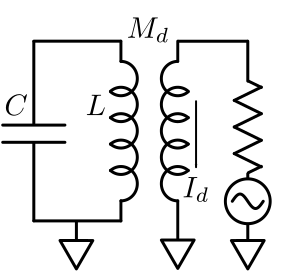
\includegraphics[width=5cm]{inductive_drive.pdf}
\par\end{centering}
  \caption{Parallel LC driving through a mutual inductance.}
\label{fig:qubits.inductive_drive}
\end{figure}

We now consider the case in which we drive by applying current into an inductor which is coupled to the qubit inductor through a mutual inductance $M$, as shown in Figure \ref{fig:qubits.inductive_drive}.
With a drive current $I_d(t)$ Kirchhoff's law for the circuit yields the equation of motion
\begin{equation}
\ddot{\Phi} + \omega_{LC}^2 \Phi = I_d \omega_{LC}^2 M \, .
\end{equation}
This equation is reproduced by the Lagrangian
\begin{equation}
\mathcal{L} = \frac{1}{2}C \dot{\Phi}^2 - \frac{1}{2L} \Phi^2 + \frac{M}{L}I_d(t) \Phi \, .
\end{equation}
The momentum conjugate to $\Phi$ is
\begin{equation}
p = \frac{\partial \mathcal{L}}{\partial \dot{\Phi}} = C \dot{\Phi} = Q
\end{equation}
and the Hamiltonian is
\begin{equation}
H = p \dot{\Phi} - \mathcal{L} = \frac{Q^2}{2C} + \frac{\Phi^2}{2L} - \frac{M}{L} I_d(t) \Phi
\end{equation}
so the driving Hamiltonian is
\begin{equation}
H_d = - \frac{M}{L}I_d(t) \Phi \, .
\end{equation}
Note that adding a parallel junction to the circuit does \emph{not} change the form of $H_d$; the junction adds a term $(I_c \Phi_0 / 2\pi)\cos(\pi \Phi / \Phi_0)$ to the Lagrangian, but this term does not couple to $I_d$.

Restricting to the lowest two levels, $H_d$ becomes
\begin{align}
H_d
&= - \frac{M}{L} I_d(t) \left(
{\begin{array}{cc} \bbraket{0}{\Phi}{0} & \bbraket{0}{\Phi}{1} \\ \bbraket{1}{\Phi}{0} & \bbraket{1}{\Phi}{1} \end{array}}
\right) \\
&= - \frac{M}{L} I_d(t) \times \nonumber \\
&\left[
\left| \Phi_{10} \right| \sigma_x
+ \frac{(\Phi_{00} - \Phi_{11})}{2} \sigma_z
+ \frac{(\Phi_{00} + \Phi_{11})}{2} \mathbf{I}
\right] \, .
\end{align}
If the circuit is nearly harmonic then $\Phi_{ii} \approx 0$ and we can re-express $\Phi$ as (see \citeinternaltype \citeinternalref{quantumOscillator})
\begin{equation}
\Phi = \Phi_{\text{zpf}} \left( a + a^\dagger \right)
\end{equation}
where $\Phi_{\text{zpf}} \equiv \sqrt{\hbar Z_{LC} / 2}$ and $Z_{LC} \equiv \sqrt{L/C}$.
Inserting this into $H_d$ gives
\begin{equation}
H_d = -\frac{M}{L} I_d(t) \Phi_{\text{zpf}} (a + a^\dagger) \, .
\end{equation}
In a two level approximation for the qubit, $(a + a^\dagger)\rightarrow \sigma_x$ and $H_d$ becomes
\begin{equation}
\text{(harmonic limit)} \quad H_d = - \frac{M}{L} I_d(t) \Phi_{\text{zpf}} \sigma_x \, .
\end{equation}
